\section{Editor}

Di seguito vengono elencati i casi d'uso per l'editor.

\subsection{Casi d'Uso}


\subsubsection{UC-E0}

    \begin{figure}[H]
      \begin{center}
        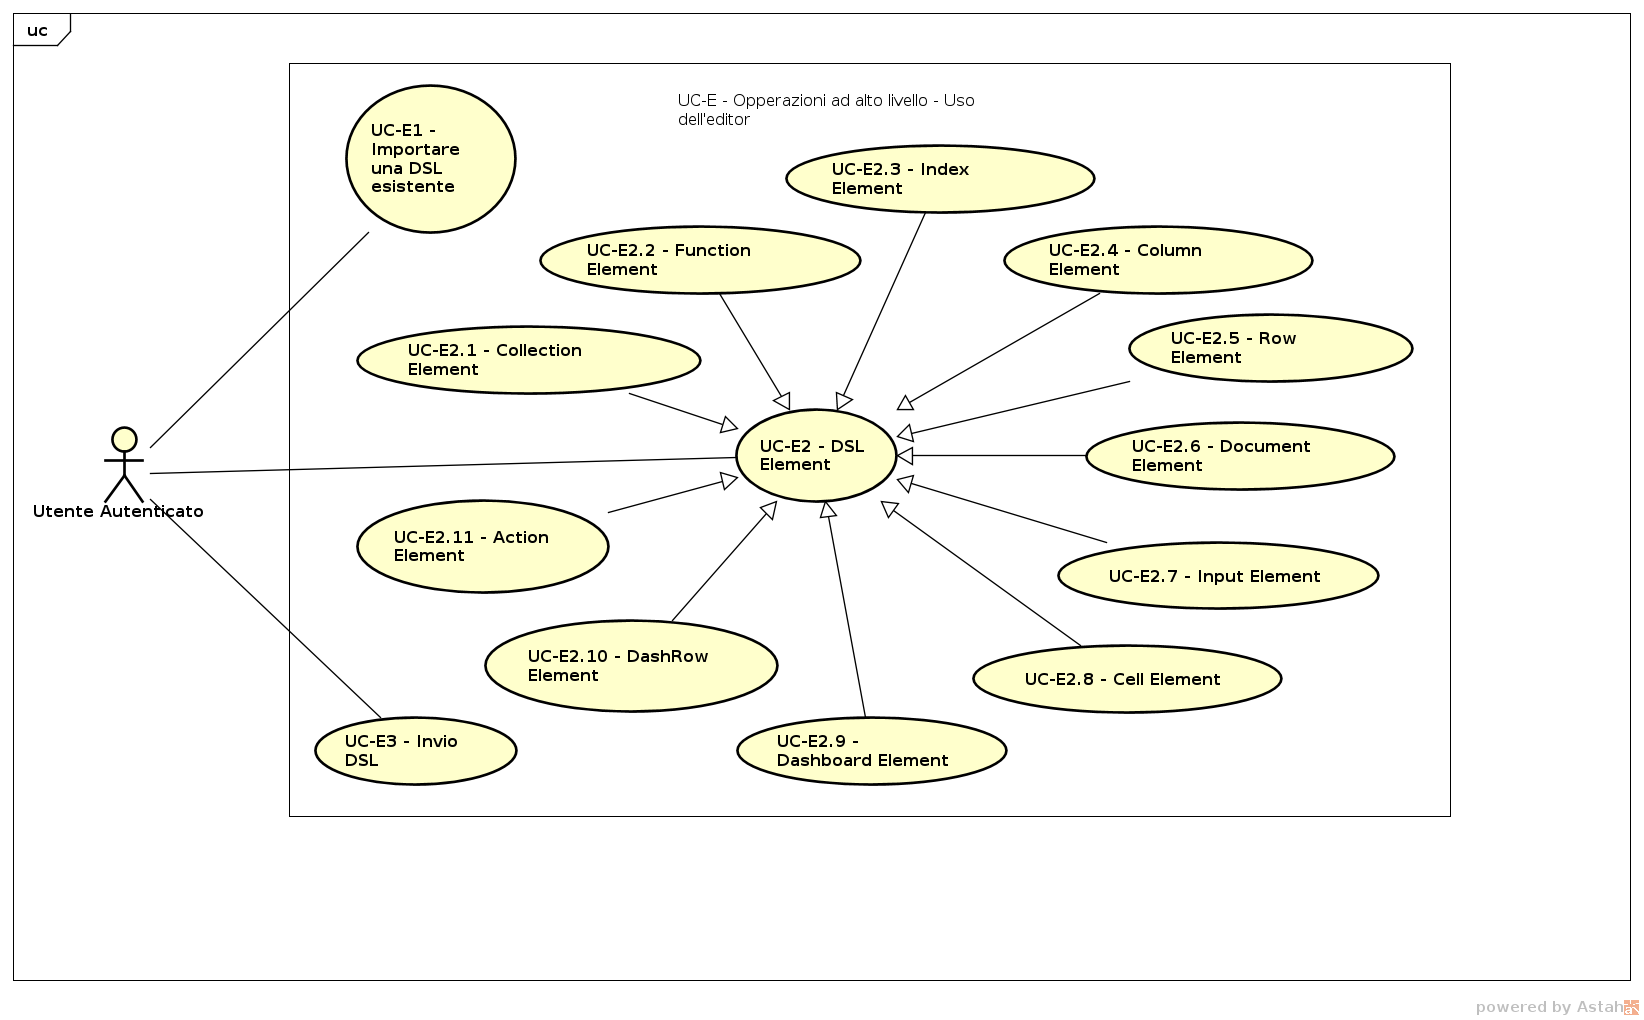
\includegraphics[width=12cm]{res/img/UCEditor/UC-E}
      \caption{UC-E0 - Operazioni ad alto livello - Uso dell'editor}
      \end{center} 
    \end{figure}    
    
    %Tabella 
    \begin{center}
      \bgroup
      \def\arraystretch{1.8}     
      \begin{longtable}{  p{3.5cm} | p{8cm} } 
        
        \hline
        \multicolumn{2}{ | c | }{ \cellcolor[gray]{0.9} \textbf{UC-E0 - Operazioni ad alto livello - Uso dell'editor}} \\ 
        \hline
        
        \textbf{Attori Primari} & Utente Autenticato, Ospite, Membro, Admin, Proprietario \\ 
        \textbf{Scopo e Descrizione} & 1. Importazione di un \textit{DSL} esitente (UC-E1)
2. Manipolazione del DSL Element tramite l'interfaccia grafica dell'editor
3. Invio del DSL al server di MaaS \\ 
        
        \textbf{Precondizioni}  & L'utente sta visualizzando l'editor e si appresta ad utilizzato \\ 
        
        \textbf{Postcondizioni} & L'utente ha utilizzato l'editor ed ha eseguito le azioni volute \\ 
        \textbf{Scenario principale} & 1. Importare un DSL esistente
2. DSL element
3. Invio di un DSL
      \end{longtable}
      \egroup
    \end{center}

    \subsubsection{UC-E1}    
    
    %Tabella 
    \begin{center}
      \bgroup
      \def\arraystretch{1.8}     
      \begin{longtable}{  p{3.5cm} | p{8cm} } 
        
        \hline
        \multicolumn{2}{ | c | }{ \cellcolor[gray]{0.9} \textbf{UC-E1 - Importare una DSL Esistente}} \\ 
        \hline
        
        \textbf{Attori Primari} & Utente Autenticato, Ospite, Membro, Admin, Proprietario \\ 
        \textbf{Scopo e Descrizione} & Importare una DSL precedentemente creato dall'utente in MaaS \\ 
        
        \textbf{Precondizioni}  & L'utente sta visualizzando l'editor e ha una DSL da importare \\ 
        
        \textbf{Postcondizioni} & L'utente ha importato con successo una DSL all'interno di MaaS
      \end{longtable}
      \egroup
    \end{center} 


\subsubsection{UC-E2}

    \begin{figure}[H]
      \begin{center}
        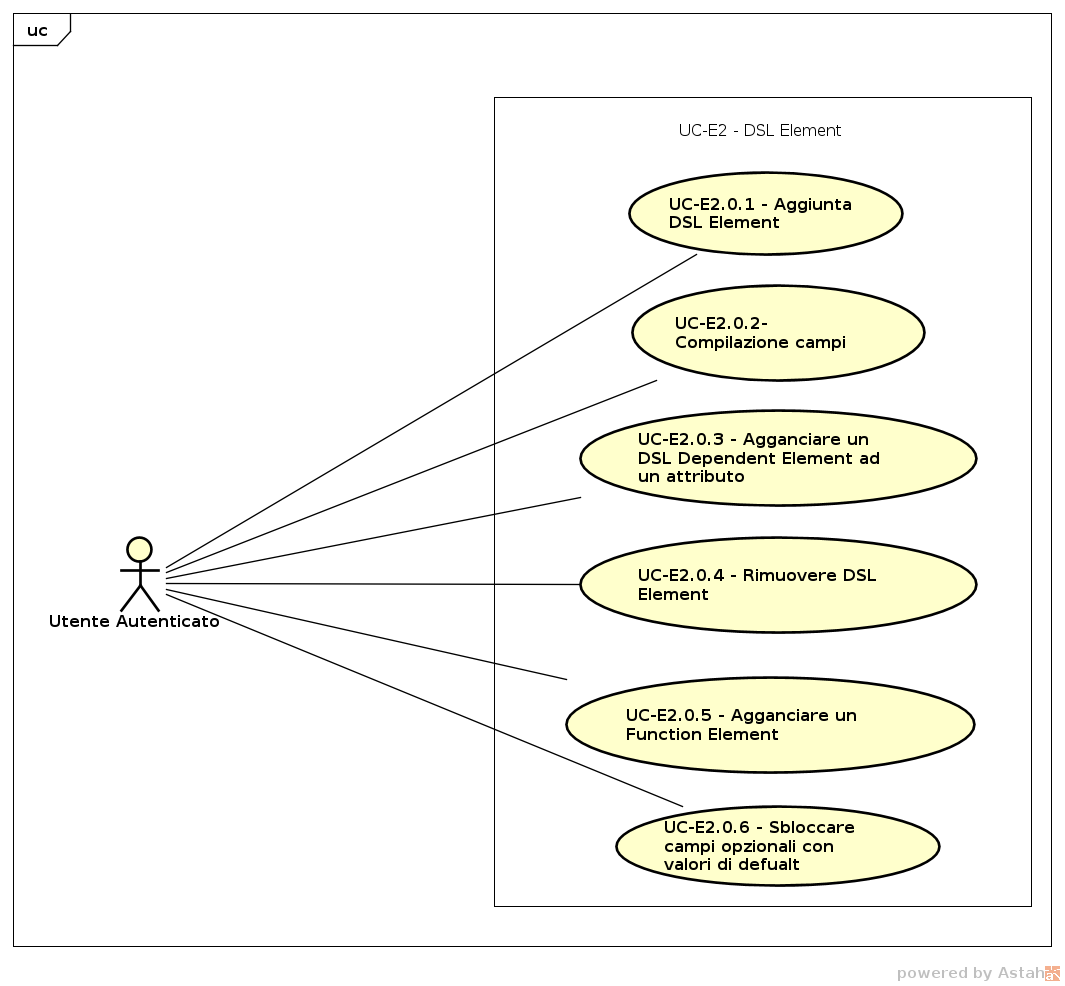
\includegraphics[width=12cm]{res/img/UCEditor/UC-E2-DSLElement}
      \caption{UC-E2 - DSL Element}
      \end{center} 
    \end{figure}    
    
    %Tabella 
    \begin{center}
      \bgroup
      \def\arraystretch{1.8}     
      \begin{longtable}{  p{3.5cm} | p{8cm} } 
        
        \hline
        \multicolumn{2}{ | c | }{ \cellcolor[gray]{0.9} \textbf{UC-E2 - DSL Element}} \\ 
        \hline
        
        \textbf{Attori Primari} & Utente Autenticato, Ospite, Membro, Admin, Proprietario \\ 
        \textbf{Scopo e Descrizione} & Il DSL Element è la zona dove è possibile aggiungere, agganciare, sbloccare o rimuovere altri elementi sul DSL. È possibile anche la compilazione dei campi. \\ 
        
        \textbf{Precondizioni}  & L'utente sta per eseguire una delle azioni elencate nello Scopo di modifica sul DSL \\ 
        
        \textbf{Postcondizioni} & L'utente ha eseguito le sue operazioni sul DSL Element con successo \\ 
        \textbf{Scenario Principale} & 1. Aggiunta DSL Element (UC-E2.0.1)
2. Compilazione campi (UC-E2.0.2)
3. Agganciare un DSL Dependent Element ad un attributo (UC-E2.0.3)
4. Rimuovere DSL Element (UC-E2.0.4)
5. Agganciare un Function Element (UC-E2.0.5)
6. Sbloccare campi opzionali con valori di default (UC-E2.0.6)
      \end{longtable}
      \egroup
    \end{center} 


\subsubsection{UC-E2.0.1}   
    
    %Tabella 
    \begin{center}
      \bgroup
      \def\arraystretch{1.8}     
      \begin{longtable}{  p{3.5cm} | p{8cm} } 
        
        \hline
        \multicolumn{2}{ | c | }{ \cellcolor[gray]{0.9} \textbf{UC-E2.0.1 - Aggiunta DSL Element}} \\ 
        \hline
        
        \textbf{Attori Primari} & Utente Autenticato, Ospiete, Membro, Admin, Proprietario \\ 
        \textbf{Scopo e Descrizione} & L'utente ha la possibiltà di aggiungere un DSL Element e di deciderne il tipo. Con DSL Element si intende la rappresentazione sull'editor di una struttura che compone il DSL. \\ 
        
        \textbf{Precondizioni}  & L'utente visualizza l'editor \\ 
        
        \textbf{Postcondizioni} & L'utente ha aggiunto con successo un DSL Element
      \end{longtable}
      \egroup
    \end{center} 
\subsubsection{UC-E2.0.2}

    %Tabella 
    \begin{center}
      \bgroup
      \def\arraystretch{1.8}     
      \begin{longtable}{  p{3.5cm} | p{8cm} } 
        
        \hline
        \multicolumn{2}{ | c | }{ \cellcolor[gray]{0.9} \textbf{UC-E2.0.2 - Compilazione campi}} \\ 
        \hline
        
        \textbf{Attori Primari} & Utente Autenticato, Ospite, Membro, Admin, Proprietario \\ 
        \textbf{Scopo e Descrizione} & L'utente ha la possibilit\`a di compilare i campi con del testo \\ 
        
        \textbf{Precondizioni}  & L'utente visualizza l'editor \\ 
        
        \textbf{Postcondizioni} & I campi desiderati dall'utente sono stati compilati con successo
      \end{longtable}
      \egroup
    \end{center}
\subsubsection{UC-E2.0.3}

    %Tabella 
    \begin{center}
      \bgroup
      \def\arraystretch{1.8}     
      \begin{longtable}{  p{3.5cm} | p{8cm} } 
        
        \hline
        \multicolumn{2}{ | c | }{ \cellcolor[gray]{0.9} \textbf{UC-E2.0.3 - Agganciare un DSL Dependent Element ad un attributo}} \\ 
        \hline
        
        \textbf{Attori Primari} & Utente Autenticato, Ospiete, Membro, Admin, Proprietario \\ 
        \textbf{Scopo e Descrizione} & Si da la possibilit\`a di agganciare un DSL Dependent Element ad un attributo. Questa azione \`e ripetibile diverse volte \\ 
        
        \textbf{Precondizioni}  & L'utente ha a disposizione un attributo e un DSL Dependent Element \\ 
        
        \textbf{Postcondizioni} & L'utente ha collegato con successo l'atributo e il DSL Dependent Element a disposizione
      \end{longtable}
      \egroup
    \end{center}
\subsubsection{UC-E2.0.4}

    %Tabella 
    \begin{center}
      \bgroup
      \def\arraystretch{1.8}     
      \begin{longtable}{  p{3.5cm} | p{8cm} } 
        
        \hline
        \multicolumn{2}{ | c | }{ \cellcolor[gray]{0.9} \textbf{UC-E2.0.4 - Rimuovere DSL Element}} \\ 
        \hline
        
        \textbf{Attori Primari} & Utente Autenticato, Ospite, Membro, Admin, Proprietario \\ 
        \textbf{Scopo e Descrizione} & \`E possibile rimuovere un DSL Element non pi\`u utilizzato o non pi\`u voluto dal DSL \\ 
        
        \textbf{Precondizioni}  & L'utente sta visualizzando l'editor e il DSL Element che vuole eliminare esiste ed \`e modificabile \\ 
        
        \textbf{Postcondizioni} & L'utente ha eliminato con successo il DSL Element 
      \end{longtable}
      \egroup
    \end{center}
\subsubsection{UC-E2.0.5}

    %Tabella 
    \begin{center}
      \bgroup
      \def\arraystretch{1.8}     
      \begin{longtable}{  p{3.5cm} | p{8cm} } 
        
        \hline
        \multicolumn{2}{ | c | }{ \cellcolor[gray]{0.9} \textbf{UC-E2.0.5 - Agganciare un Function Element}} \\ 
        \hline
        
        \textbf{Attori Primari} & Utente Autenticato, Ospite, Membro, Admin, Proprietario \\ 
        \textbf{Scopo e Descrizione} & L'intento \`e quello di dare la possibilit\`a all'utilizzatore dell'editor di poter agganciare un Function Element a qualche suo attributo. Con Function Element si esprime la rappresentazione di una funzione nel linguaggio di rappresentazione adottato \\ 
        
        \textbf{Precondizioni}  & L'utente sta visualizzando l'editor e dispone di una Function Element collegabile \\ 
        
        \textbf{Postcondizioni} & L'utente ha agganciato con successo la Function Element
      \end{longtable}
      \egroup
    \end{center}
\subsubsection{UC-E2.0.6}

    %Tabella 
    \begin{center}
      \bgroup
      \def\arraystretch{1.8}     
      \begin{longtable}{  p{3.5cm} | p{8cm} } 
        
        \hline
        \multicolumn{2}{ | c | }{ \cellcolor[gray]{0.9} \textbf{UC-E2.0.6 - Sbloccare campi opzionali con valori di default}} \\ 
        \hline
        
        \textbf{Attori Primari} & Utente Autenticato, Ospite, Membro, Admin, Proprietario \\ 
        \textbf{Scopo e Descrizione} & Si da la possibilit\`a di sbloccare campi opzionali nel DSL assegnandogli valori di default \\ 
        
        \textbf{Precondizioni}  & L'utente ha la possibilit\`a di creare campi opzionali con valori di default \\ 
        
        \textbf{Postcondizioni} & L'utente ha creato campi opzionali con valori di default
      \end{longtable}
      \egroup
    \end{center}
\subsubsection{UC-E2.1}
 

    \begin{figure}[H]
      \begin{center}
        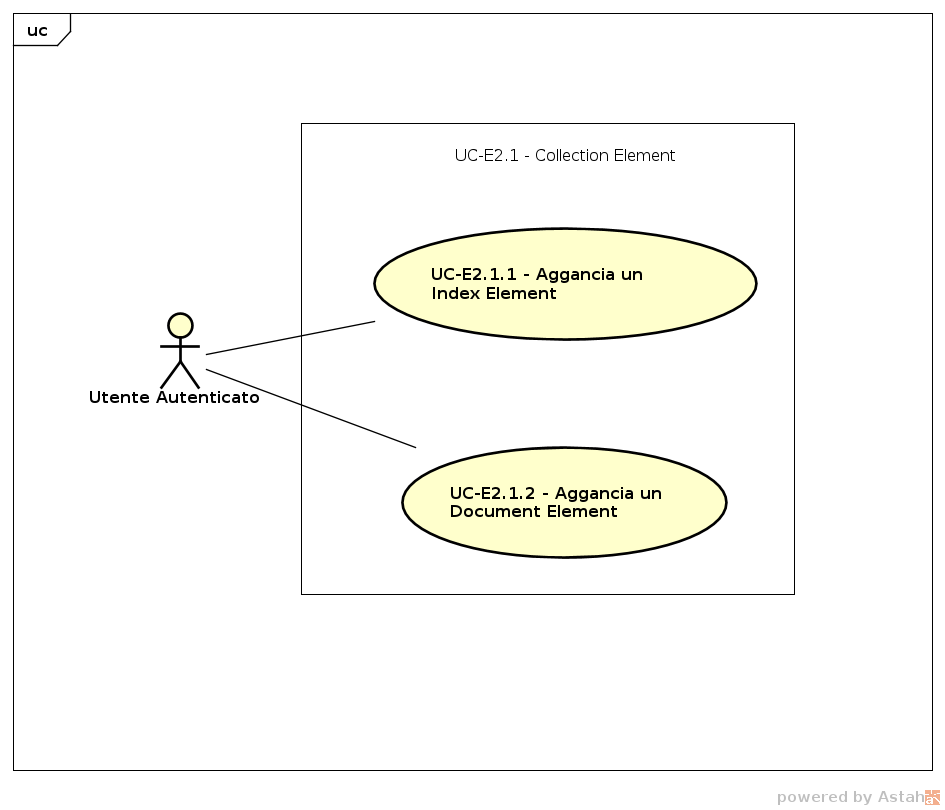
\includegraphics[width=12cm]{res/img/UCEditor/UC-E2.1-CollectionElement}
      \caption{UC-E2.1 - Collection Element}
      \end{center} 
    \end{figure}

    %Tabella 
    \begin{center}
      \bgroup
      \def\arraystretch{1.8}     
      \begin{longtable}{  p{3.5cm} | p{8cm} } 
        
        \hline
        \multicolumn{2}{ | c | }{ \cellcolor[gray]{0.9} \textbf{UC-E2.1 - Collection Element}} \\ 
        \hline
        
        \textbf{Attori Primari} & Utente Autenticato, Ospite, Membro, Admin, Proprietario \\ 
        \textbf{Scopo e Descrizione} & Rappresentazione della sezione della parte della collection del DSL \\ 
        
        \textbf{Precondizioni}  & L'utente sta visualizzando l'editor \\ 
        
        \textbf{Postcondizioni} & L'utente ha manipolato la \textit{Collection} del \textit{DSL} \\ 
        \textbf{Scenario principale} & 1. Aggancia un Index Element (UC-E2.1.1)
2. Aggancia un Document Element (UC-E2.1.2) \\
\end{longtable}
      \egroup
    \end{center}
\subsubsection{UC-E2.1.1}

    %Tabella 
    \begin{center}
      \bgroup
      \def\arraystretch{1.8}     
      \begin{longtable}{  p{3.5cm} | p{8cm} } 
        
        \hline
        \multicolumn{2}{ | c | }{ \cellcolor[gray]{0.9} \textbf{UC-E2.1.1 - Aggancia un Index Element}} \\ 
        \hline
        
        \textbf{Attori Primari} & Utente Autenticato, Ospite, Membro, Admin, Proprietario \\ 
        \textbf{Scopo e Descrizione} & Unire alla collection creata un elemento Index del DSL \\ 
        
        \textbf{Precondizioni}  & La Collection esiste o \`e appena stata creata \\ 
        
        \textbf{Postcondizioni} & Un Index Element \`e stato agganciato a una Collection
      \end{longtable}
      \egroup
    \end{center}
\subsubsection{UC-E2.1.2}

    %Tabella 
    \begin{center}
      \bgroup
      \def\arraystretch{1.8}     
      \begin{longtable}{  p{3.5cm} | p{8cm} } 
        
        \hline
        \multicolumn{2}{ | c | }{ \cellcolor[gray]{0.9} \textbf{UC-E2.1.2 - Aggancia un Document Element}} \\ 
        \hline
        
        \textbf{Attori Primari} & Utente Autenticato, Ospite, Membro, Admin, Proprietario \\ 
        \textbf{Scopo e Descrizione} & Inserisce la sezione Show relativa alla collection creata nel DSL \\ 
        
        \textbf{Precondizioni}  & L'utente visualizza l'editor \\ 
        
        \textbf{Postcondizioni} & L'utente ha con successo agganciato una Show al Document Element 
      \end{longtable}
      \egroup
    \end{center}
\subsubsection{UC-E2.2}
 

    \begin{figure}[H]
      \begin{center}
        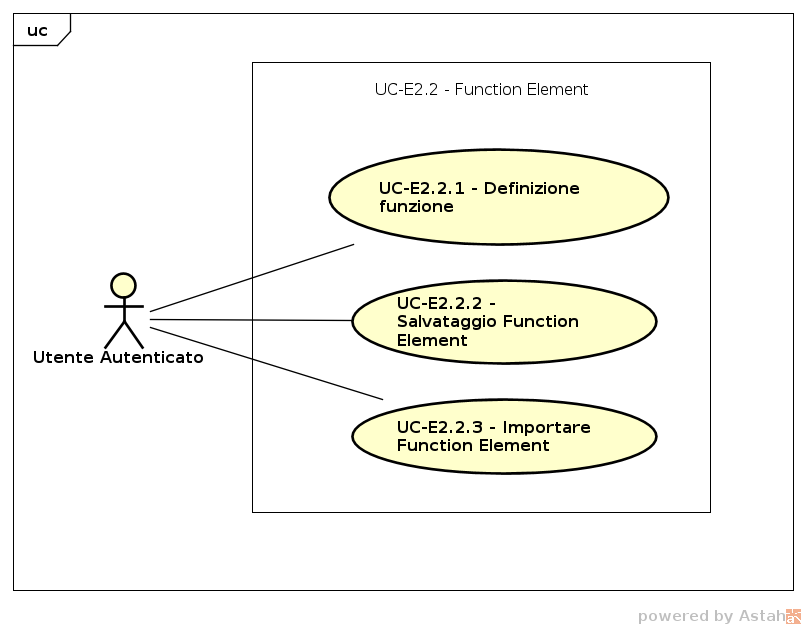
\includegraphics[width=12cm]{res/img/UCEditor/UC-E2.2-FunctionElement}
      \caption{UC-E2.2 - Function Element}
      \end{center} 
    \end{figure}

    %Tabella 
    \begin{center}
      \bgroup
      \def\arraystretch{1.8}     
      \begin{longtable}{  p{3.5cm} | p{8cm} } 
        
        \hline
        \multicolumn{2}{ | c | }{ \cellcolor[gray]{0.9} \textbf{UC-E2.2 - Function Element}} \\ 
        \hline
        
        \textbf{Attori Primari} & Utente Autenticato, Ospite, Membro, Admin, Proprietario \\ 
        \textbf{Scopo e Descrizione} & Viene data la possibilit\`a all'utente di creare 
            una funzione di collegamento tra gli elementi del \textit{DSL}. \\ 
        
        \textbf{Precondizioni}  & L'editor \`e pronto per l'utilizzo \\ 
        
        \textbf{Postcondizioni} & L'utente ha collegato un \textit{function element} al valore del DSL desiderato \\ 
        \textbf{Scenario principale} & 1. Definizione di un \textit{function element} (UC-E2.2.1)
2. Salvataggio Function Element (UC-E2.2.2)
3. Importare Function Element (UC-E2.2.3)  \\
      \end{longtable}
      \egroup
    \end{center}
\subsubsection{UC-E2.2.1}

    %Tabella 
    \begin{center}
      \bgroup
      \def\arraystretch{1.8}     
      \begin{longtable}{  p{3.5cm} | p{8cm} } 
        
        \hline
        \multicolumn{2}{ | c | }{ \cellcolor[gray]{0.9} \textbf{UC-E2.2.1 - Definizione funzione}} \\ 
        \hline
        
        \textbf{Attori Primari} & Utente Autenticato, Ospite, Membro, Admin, Proprietario \\ 
        \textbf{Scopo e Descrizione} & L'utente ha la possibilit\`a di scrivere in un campo di testo una funzione nella sintassi del \textit{DSL}. \\ 
        
        \textbf{Precondizioni}  & L'utente sta visualizzando l'editor \\ 
        
        \textbf{Postcondizioni} & L'utente ha definito con successo una funzione
      \end{longtable}
      \egroup
    \end{center}
\subsubsection{UC-E2.2.2}

    %Tabella 
    \begin{center}
      \bgroup
      \def\arraystretch{1.8}     
      \begin{longtable}{  p{3.5cm} | p{8cm} } 
        
        \hline
        \multicolumn{2}{ | c | }{ \cellcolor[gray]{0.9} \textbf{UC-E2.2.2 - Salvataggio Function Element}} \\ 
        \hline
        
        \textbf{Attori Primari} & Utente Autenticato, Ospite, Membro, Admin, Proprietario \\ 
        \textbf{Scopo e Descrizione} & L'utente ha la possibilit\`a di storicizzare la sua Function Element creata \\ 
        
        \textbf{Precondizioni}  & L'utente ha inserito una Function Element valida \\ 
        
        \textbf{Postcondizioni} & La Function Element \`e stata salvata con successo in MaaS
      \end{longtable}
      \egroup
    \end{center}
\subsubsection{UC-E2.2.3}

    %Tabella 
    \begin{center}
      \bgroup
      \def\arraystretch{1.8}     
      \begin{longtable}{  p{3.5cm} | p{8cm} } 
        
        \hline
        \multicolumn{2}{ | c | }{ \cellcolor[gray]{0.9} \textbf{UC-E2.2.3 - Importare Function Element}} \\ 
        \hline
        
        \textbf{Attori Primari} & Utente Autenticato, Ospite, Membro, Admin, Proprietario \\ 
        \textbf{Scopo e Descrizione} & Il sistema permette di importare un \textit{Function Element} precedentemente definito nella sessione corrente.\\ 
        
        \textbf{Precondizioni}  & Il sistema fornisce i \textit{Function Element} precedentemente definiti. \\ 
        
        \textbf{Postcondizioni} & L'utente ha caricato la Function Element con successo. \\ 
      \end{longtable}
      \egroup
    \end{center}
\subsubsection{UC-E2.3}
 

    \begin{figure}[H]
      \begin{center}
        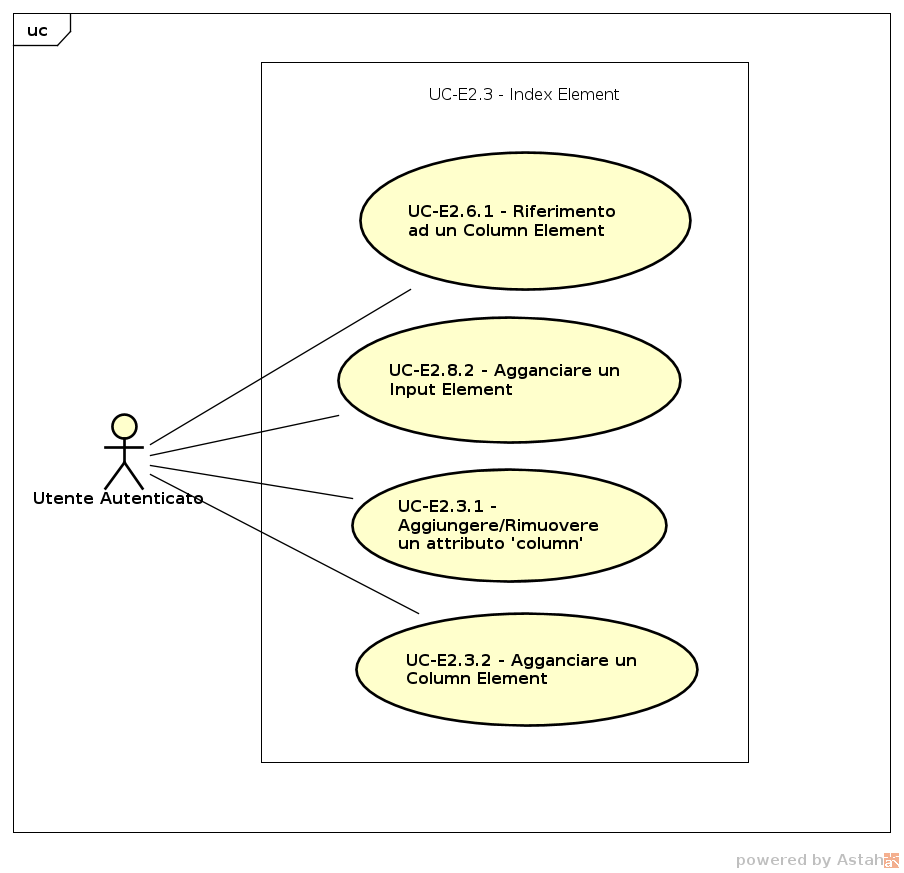
\includegraphics[width=12cm]{res/img/UCEditor/UC-E2.3-IndexElement}
      \caption{UC-E2.3 - Index Element}
      \end{center} 
    \end{figure}

    %Tabella 
    \begin{center}
      \bgroup
      \def\arraystretch{1.8}     
      \begin{longtable}{  p{3.5cm} | p{8cm} } 
        
        \hline
        \multicolumn{2}{ | c | }{ \cellcolor[gray]{0.9} \textbf{UC-E2.3 - Index Element}} \\ 
        \hline
        
        \textbf{Attori Primari} & Utente Autenticato, Ospite, Membro, Admin, Proprietario \\ 
        \textbf{Scopo e Descrizione} & Rappresentazione della sezione index del DSL nell'editor \\ 
        
        \textbf{Precondizioni}  & L'aggiunta dell'Index Element dev'essere eseguita in una Collection Element esistente \\ 
        
        \textbf{Postcondizioni} & \`E stata aggiunta la sezione Index alla Collection del DSL corrente \\ 
        \textbf{Scenario Principale} & 1. Riferimento ad un Column Element (UC-E2.6.1)
2. Collegare un Input Element (UC-E2.8.2)
3. Aggiungere/Rimuovere un attributo ``column'' (UC-E2.3.1)
4. Collegare un Column Element (UC-E2.3.2)
      \end{longtable}
      \egroup
    \end{center}
\subsubsection{UC-E2.3.1}

    %Tabella 
    \begin{center}
      \bgroup
      \def\arraystretch{1.8}     
      \begin{longtable}{  p{3.5cm} | p{8cm} } 
        
        \hline
        \multicolumn{2}{ | c | }{ \cellcolor[gray]{0.9} \textbf{UC-E2.3.1 - Aggiungere/Rimuovere un attributo ``column''}} \\ 
        \hline
        
        \textbf{Attori Primari} & Utente Autenticato, Ospite, Membro, Admin, Proprietario \\ 
        \textbf{Scopo e Descrizione} & Si da la possibilit\`a di rimuovere o aggiungere dall'Index un attributo \\ 
        
        \textbf{Precondizioni}  & Sia collegata a un Index Element \\ 
        
        \textbf{Postcondizioni} & Nel DSL nella sezione Index \`e aggiunto o rimosso un attributo ``column'' 
      \end{longtable}
      \egroup
    \end{center}
\subsubsection{UC-E2.3.2}

    %Tabella 
    \begin{center}
      \bgroup
      \def\arraystretch{1.8}     
      \begin{longtable}{  p{3.5cm} | p{8cm} } 
        
        \hline
        \multicolumn{2}{ | c | }{ \cellcolor[gray]{0.9} \textbf{UC-E2.3.2 - Collegare un \textit{Column Element}}} \\ 
        \hline
        
        \textbf{Attori Primari} & Utente Autenticato, Ospite, Membro, Admin, Proprietario \\ 
        \textbf{Scopo e Descrizione} & \`E possibile agganciare un Column Element all'attributo ``column'' \\ 
        
        \textbf{Precondizioni}  & Deve essere presente un attributo Column \\ 
        
        \textbf{Postcondizioni} & La sezione del DSL ``column'' viene riempita con i valori impostati sul Column Element  
      \end{longtable}
      \egroup
    \end{center}
\subsubsection{UC-E2.4}

    %Tabella 
    \begin{center}
      \bgroup
      \def\arraystretch{1.8}     
      \begin{longtable}{  p{3.5cm} | p{8cm} } 
        
        \hline
        \multicolumn{2}{ | c | }{ \cellcolor[gray]{0.9} \textbf{UC-E2.4 - Column Element}} \\ 
        \hline
        
        \textbf{Attori Primari} & Utente Autenticato, Ospite, membro, Admin, Proprietario \\ 
        \textbf{Scopo e Descrizione} & Dare tutte le funzionalit\`a espresse nel DSL Element \\ 
        
        \textbf{Precondizioni}  & Deve riferirsi ad una struttura column presente nel DSL corrente \\ 
        
        \textbf{Postcondizioni} & L'utente manipola le parti che compongono la struttura 
      \end{longtable}
      \egroup
    \end{center}
\subsubsection{UC-E2.5}

    %Tabella 
    \begin{center}
      \bgroup
      \def\arraystretch{1.8}     
      \begin{longtable}{  p{3.5cm} | p{8cm} } 
        
        \hline
        \multicolumn{2}{ | c | }{ \cellcolor[gray]{0.9} \textbf{UC-E2.5 - Row Element}} \\ 
        \hline
        
        \textbf{Attori Primari} & Utente Autenticato, Ospite, Membro, Admin, Proprietario \\ 
        \textbf{Scopo e Descrizione} & Rappresentazione di una struttura Row all'interno del DSL \\ 
        
        \textbf{Precondizioni}  & Dev'essere legata a una struttura Document \\ 
        
        \textbf{Postcondizioni} & Viene definita la struttura della Row all'interno del DSL corrente 
      \end{longtable}
      \egroup
    \end{center}
\subsubsection{UC-E2.6}
 

    \begin{figure}[H]
      \begin{center}
        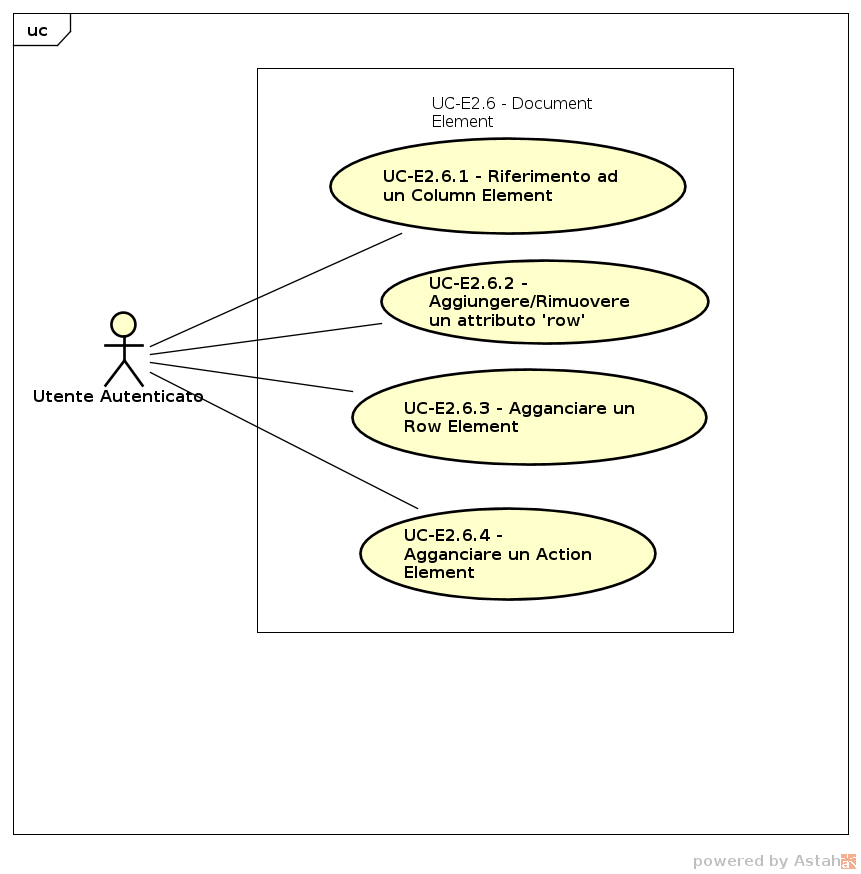
\includegraphics[width=12cm]{res/img/UCEditor/UC-E2.6-DocumentElement}
      \caption{UC-E2.6 - Document Element}
      \end{center} 
    \end{figure}

    %Tabella 
    \begin{center}
      \bgroup
      \def\arraystretch{1.8}     
      \begin{longtable}{  p{3.5cm} | p{8cm} } 
        
        \hline
        \multicolumn{2}{ | c | }{ \cellcolor[gray]{0.9} \textbf{UC-E2.6 - Document Element}} \\ 
        \hline
        
        \textbf{Attori Primari} & Utente Autenticato, Ospite, Membro, Admin, Proprietario \\ 
        \textbf{Scopo e Descrizione} & Rappresenta l'elemento Document del DSL \\ 
        
        \textbf{Precondizioni}  & L'utente visualizza l'editor \\ 
        
        \textbf{Postcondizioni} & Viene generato l'elemento Document nel DSL \\ 
        \textbf{Scenario Principale} & 1. Riferimento ad un Column Element (UC-E2.6.1)
2. Aggiungere/Rimuovere un attributo row (UC-E2.6.2)
3. Agganciare un Row Element (UC-E2.6.3)
4. Agganciare un Action Element (UC-E2.6.4) 
      \end{longtable}
      \egroup
    \end{center}
\subsubsection{UC-E2.6.1}

    %Tabella 
    \begin{center}
      \bgroup
      \def\arraystretch{1.8}     
      \begin{longtable}{  p{3.5cm} | p{8cm} } 
        
        \hline
        \multicolumn{2}{ | c | }{ \cellcolor[gray]{0.9} \textbf{UC-E2.6.1 - Riferimento ad un Column Element}} \\ 
        \hline
        
        \textbf{Attori Primari} & Utente Autenticato, Ospite, Membro, Admin, Proprietario \\ 
        \textbf{Scopo e Descrizione} & Riferirsi ad un elemento colonna precedentemente definito in modo da applicare la populate del DSL \\ 
        
        \textbf{Precondizioni}  & Esista almeno un elemento Document a cui si riferisca \\ 
        
        \textbf{Postcondizioni} & Viene composta la funzione populate
      \end{longtable}
      \egroup
    \end{center}
\subsubsection{UC-E2.6.2}

    %Tabella 
    \begin{center}
      \bgroup
      \def\arraystretch{1.8}     
      \begin{longtable}{  p{3.5cm} | p{8cm} } 
        
        \hline
        \multicolumn{2}{ | c | }{ \cellcolor[gray]{0.9} \textbf{UC-E2.6.2 - Aggiungere/Rimuovere un attributo row}} \\ 
        \hline
        
        \textbf{Attori Primari} & Utente Autenticato, Ospite, Membro, Admin, Proprietario \\ 
        \textbf{Scopo e Descrizione} & Aggiungere o rimuovere una struttura ``row'' all'interno del Document nella struttura DSL \\ 
        
        \textbf{Precondizioni}  & Si deve riferire a un Document esistente \\ 
        
        \textbf{Postcondizioni} & \`E stata manipolata (aggiunta o rimossa) una ``row'' all'interno del DSL Document 
      \end{longtable}
      \egroup
    \end{center}
\subsubsection{UC-E2.6.3}

    %Tabella 
    \begin{center}
      \bgroup
      \def\arraystretch{1.8}     
      \begin{longtable}{  p{3.5cm} | p{8cm} } 
        
        \hline
        \multicolumn{2}{ | c | }{ \cellcolor[gray]{0.9} \textbf{UC-E2.6.3 - Agganciare un Row Element}} \\ 
        \hline
        
        \textbf{Attori Primari} & Utente Autenticato, Ospite, Membro, Admin, Proprietario \\ 
        \textbf{Scopo e Descrizione} & Definire la struttura della ``row'' del DSL  \\ 
        
        \textbf{Precondizioni}  & Sia presente un attributo ``row'' nel Document \\ 
        
        \textbf{Postcondizioni} & Nel DSL vengono trascritti nella struttura ``row'' gli attributi e i rispettivi valori 
      \end{longtable}
      \egroup
    \end{center}
\subsubsection{UC-E2.6.4}

    %Tabella 
    \begin{center}
      \bgroup
      \def\arraystretch{1.8}     
      \begin{longtable}{  p{3.5cm} | p{8cm} } 
        
        \hline
        \multicolumn{2}{ | c | }{ \cellcolor[gray]{0.9} \textbf{UC-E2.6.4 - Agganciare un Action Element}} \\ 
        \hline
        
        \textbf{Attori Primari} & Utente Autenticato, Ospite, Membro, Admin, Proprietario \\ 
        \textbf{Scopo e Descrizione} & Legare il contenuto informativo della ``row'' all'azione definita dalla ``action'' \\ 
        
        \textbf{Precondizioni}  & \`E definita una ``row'' all'interno del DSL \\ 
        
        \textbf{Postcondizioni} & Verr\`a definita la ``action'' nella ``row'' 
      \end{longtable}
      \egroup
    \end{center}
\subsubsection{UC-E2.7}
 

    \begin{figure}[H]
      \begin{center}
        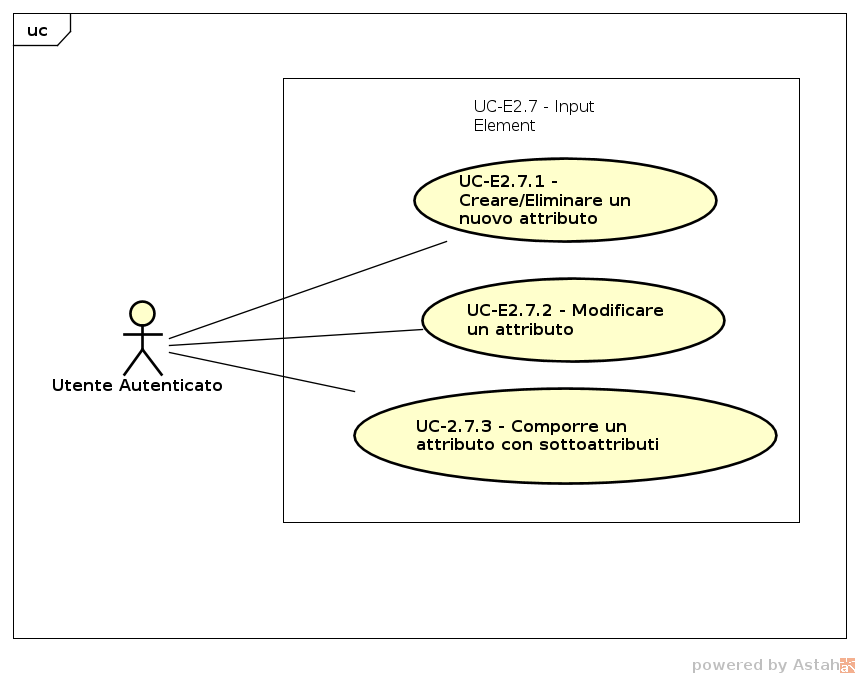
\includegraphics[width=12cm]{res/img/UCEditor/UC-E2.7-InputElement}
      \caption{UC-E2.7 - Input Element}
      \end{center} 
    \end{figure}

    %Tabella 
    \begin{center}
      \bgroup
      \def\arraystretch{1.8}     
      \begin{longtable}{  p{3.5cm} | p{8cm} } 
        
        \hline
        \multicolumn{2}{ | c | }{ \cellcolor[gray]{0.9} \textbf{UC-E2.7 - Input Element}} \\ 
        \hline
        
        \textbf{Attori Primari} & Utente Autenticato, Ospite, Membro, Admin, Proprietario \\ 
        \textbf{Scopo e Descrizione} & Si occupa di rappresentare una dato in un specifico formato \\ 
        
        \textbf{Precondizioni}  & L'utente pu\`o visualizzare l'Editor \\ 
        
        \textbf{Postcondizioni} & Viene composto il dato con i valori inseriti dall'utente \\ 
        \textbf{Scenario Principale} & 1. Creare/Eliminare un nuovo attributo (UC-E2.7.1)
2. Modificare un attributo (UC-E2.7.2)
3. Comporre un attributo con sottoattributi (UC-E2.7.3)
      \end{longtable}
      \egroup
    \end{center}
\subsubsection{UC-E2.7.1}

    %Tabella 
    \begin{center}
      \bgroup
      \def\arraystretch{1.8}     
      \begin{longtable}{  p{3.5cm} | p{8cm} } 
        
        \hline
        \multicolumn{2}{ | c | }{ \cellcolor[gray]{0.9} \textbf{UC-E2.7.1 - Creare/Eliminare un nuovo attributo}} \\ 
        \hline
        
        \textbf{Attori Primari} & Utente Autenticato, Ospite, Membro, Admin, Proprietario \\ 
        \textbf{Scopo e Descrizione} & Essendo il dato componibile da pi\`u attributi, permette di definire una coppia chiave/valore per meglio definire il suo dato \\ 
        
        \textbf{Precondizioni}  & L'utente si deve riferire a un Data Element presente \\ 
        
        \textbf{Postcondizioni} & Si manipola l'attributo selezionato
      \end{longtable}
      \egroup
    \end{center}
\subsubsection{UC-E2.7.2}

    %Tabella 
    \begin{center}
      \bgroup
      \def\arraystretch{1.8}     
      \begin{longtable}{  p{3.5cm} | p{8cm} } 
        
        \hline
        \multicolumn{2}{ | c | }{ \cellcolor[gray]{0.9} \textbf{UC-E2.7.2 - Modificare un attributo}} \\ 
        \hline
        
        \textbf{Attori Primari} & Utente Autenticato, Ospite, Membro, Admin, Proprietario \\ 
        \textbf{Scopo e Descrizione} & Poter rinominare o la chiave o il valore all'interno di un Data Element \\ 
        
        \textbf{Precondizioni}  & Ci sia un attributo a cui riferirsi \\ 
        
        \textbf{Postcondizioni} & Viene modificata o la chiave o il valore dell'attributo selezionato dall'utente
      \end{longtable}
      \egroup
    \end{center}
\subsubsection{UC-E2.7.3}

    %Tabella 
    \begin{center}
      \bgroup
      \def\arraystretch{1.8}     
      \begin{longtable}{  p{3.5cm} | p{8cm} } 
        
        \hline
        \multicolumn{2}{ | c | }{ \cellcolor[gray]{0.9} \textbf{UC-E2.7.3 - Comporre un attributo con sottoattributi}} \\ 
        \hline
        
        \textbf{Attori Primari} & Utente Autenticato, Ospite, Membro, Admin, Proprietario \\ 
        \textbf{Scopo e Descrizione} & Un utente \`e in grado di poter definire strutture complesse per i suoi scopi \\ 
        
        \textbf{Precondizioni}  & Ci sia un Data Element a cui riferirsi \\ 
        
        \textbf{Postcondizioni} & L'attributo del dato \`e a sua volta costituito da altri attributi
      \end{longtable}
      \egroup
    \end{center}
\subsubsection{UC-E2.8}
 

    \begin{figure}[H]
      \begin{center}
        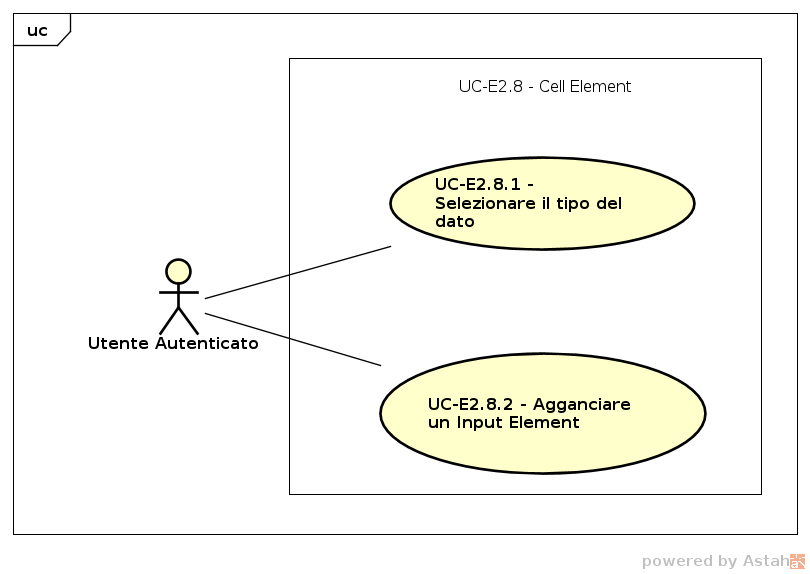
\includegraphics[width=12cm]{res/img/UCEditor/UC-E2.8-CellElement}
      \caption{UC-E2.8 - Cell Element}
      \end{center} 
    \end{figure}

    %Tabella 
    \begin{center}
      \bgroup
      \def\arraystretch{1.8}     
      \begin{longtable}{  p{3.5cm} | p{8cm} } 
        
        \hline
        \multicolumn{2}{ | c | }{ \cellcolor[gray]{0.9} \textbf{UC-E2.8 - Cell Element}} \\ 
        \hline
        
        \textbf{Attori Primari} & Utente Autenticato, Ospite, Membro, Admin, Proprietario \\ 
        \textbf{Scopo e Descrizione} & Rappresentare l'elemento Cell del DSL. \\ 
        
        \textbf{Precondizioni}  & L'utente sta visualizzando l'editor \\ 
        
        \textbf{Postcondizioni} & Viene composta l'elemento Cell nel DSL \\ 
        \textbf{Scenario Principale} &  1. Selezionare il tipo del dato (UC-E2.8.1)
2. Agganciare un Data Element (UC-E2.8.2)
      \end{longtable}
      \egroup
    \end{center}
\subsubsection{UC-E2.8.1}

    %Tabella 
    \begin{center}
      \bgroup
      \def\arraystretch{1.8}     
      \begin{longtable}{  p{3.5cm} | p{8cm} } 
        
        \hline
        \multicolumn{2}{ | c | }{ \cellcolor[gray]{0.9} \textbf{UC-E2.8.1 - Selezionare il tipo del dato}} \\ 
        \hline
        
        \textbf{Attori Primari} & Utente Autenticato, Ospite, Membro, Admin, Proprietario \\ 
        \textbf{Scopo e Descrizione} & Selezionare il tipo di dato da visualizzare, che pu\`o essere:
a. string
b. number
c. link
d. image
e. date \\ 
        
        \textbf{Precondizioni}  & Il tipo di input si deve riferire a un Cell Element \\ 
        
        \textbf{Postcondizioni} & \`E definito nel DSL il tipo di visualizzazione di dato 
      \end{longtable}
      \egroup
    \end{center}
\subsubsection{UC-E2.8.2}

    %Tabella 
    \begin{center}
      \bgroup
      \def\arraystretch{1.8}     
      \begin{longtable}{  p{3.5cm} | p{8cm} } 
        
        \hline
        \multicolumn{2}{ | c | }{ \cellcolor[gray]{0.9} \textbf{UC-E2.8.2 - Agganciare un Input Element}} \\ 
        \hline
        
        \textbf{Attori Primari} & Utente Autenticato, Ospite, Membro, Admin, Proprietario \\ 
        \textbf{Scopo e Descrizione} & Definire quale input il Cell Element rapprensenter\`a \\ 
        
        \textbf{Precondizioni}  & Ci sia un Data Element presente e un Cell Element da collegare \\ 
        
        \textbf{Postcondizioni} & Nel DSL \`e specificato quale valore il Cell Element rappresenta 
      \end{longtable}
      \egroup
    \end{center}
\subsubsection{UC-E2.9}
 

    \begin{figure}[H]
      \begin{center}
        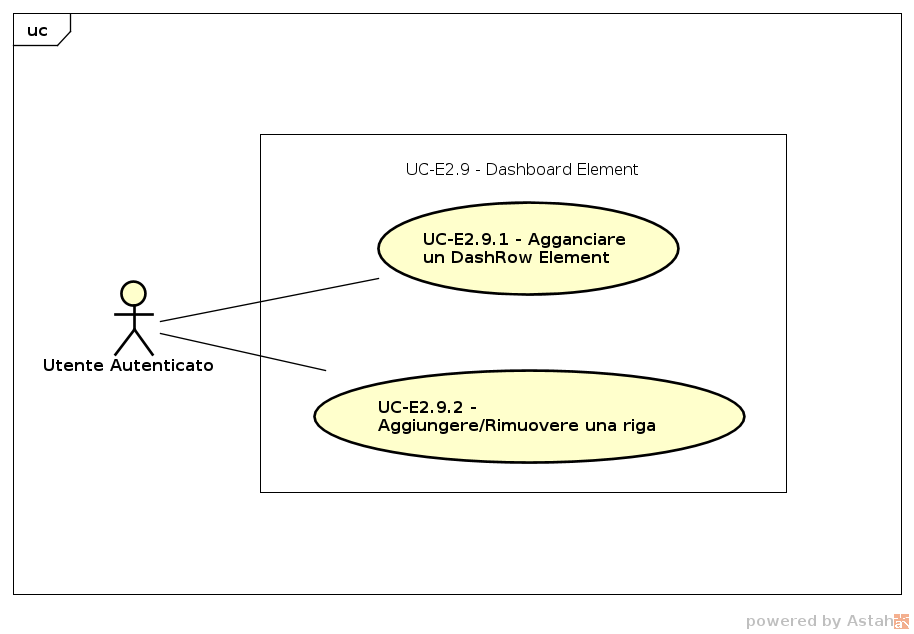
\includegraphics[width=12cm]{res/img/UCEditor/UC-E2.9-DashboardElement}
      \caption{UC-E2.9 - Dashboard Element}
      \end{center} 
    \end{figure}

    %Tabella 
    \begin{center}
      \bgroup
      \def\arraystretch{1.8}     
      \begin{longtable}{  p{3.5cm} | p{8cm} } 
        
        \hline
        \multicolumn{2}{ | c | }{ \cellcolor[gray]{0.9} \textbf{UC-E2.9 - Dashboard Element}} \\ 
        \hline
        
        \textbf{Attori Primari} & Utente Autenticato, Ospite, Membro, Admin, Proprietario \\ 
        \textbf{Scopo e Descrizione} & Rappresentazione di un elemento Dashboard nel DSL \\ 
        
        \textbf{Precondizioni}  & L'utente sta visualizzando l'editor \\ 
        
        \textbf{Postcondizioni} & Viene scritto nel DSL l'elemento Dashboard \\ 
        \textbf{Scenario Principale} & 1. Agganciare un DashRow Element (UC-E2.9.1)
2. Aggiungere/Rimuovere una riga (UC-E2.9.2)
      \end{longtable}
      \egroup
    \end{center}
\subsubsection{UC-E2.9.1}

    %Tabella 
    \begin{center}
      \bgroup
      \def\arraystretch{1.8}     
      \begin{longtable}{  p{3.5cm} | p{8cm} } 
        
        \hline
        \multicolumn{2}{ | c | }{ \cellcolor[gray]{0.9} \textbf{UC-E2.9.1 - Agganciare un DashRow Element}} \\ 
        \hline
        
        \textbf{Attori Primari} & Utente Autenticato, Ospite, Membro, Admin, Proprietario \\ 
        \textbf{Scopo e Descrizione} & Permette di definire la struttura di una Row e di legarla a una Dashboard \\ 
        
        \textbf{Precondizioni}  & Ci sia una Dashboard a cui fare riferimento \\ 
        
        \textbf{Postcondizioni} & Viene inserita nel DSL la configurazione della struttura ``row'' 
      \end{longtable}
      \egroup
    \end{center}
\subsubsection{UC-E2.9.2}

    %Tabella 
    \begin{center}
      \bgroup
      \def\arraystretch{1.8}     
      \begin{longtable}{  p{3.5cm} | p{8cm} } 
        
        \hline
        \multicolumn{2}{ | c | }{ \cellcolor[gray]{0.9} \textbf{UC-E2.9.2 - Aggiungere/Rimuovere una riga}} \\ 
        \hline
        
        \textbf{Attori Primari} & Utente Autenticato, Ospite, Membro, Admin, Proprietario \\ 
        \textbf{Scopo e Descrizione} & Definire una nuova riga all'interno della Dashboard \\ 
        
        \textbf{Precondizioni}  & Ci sia una Dashboard a cui fare riferimento \\ 
        
        \textbf{Postcondizioni} & Viene aggiunto e rimosso un attributo ``row'' 
      \end{longtable}
      \egroup
    \end{center}
\subsubsection{UC-E2.10}
 

    \begin{figure}[H]
      \begin{center}
        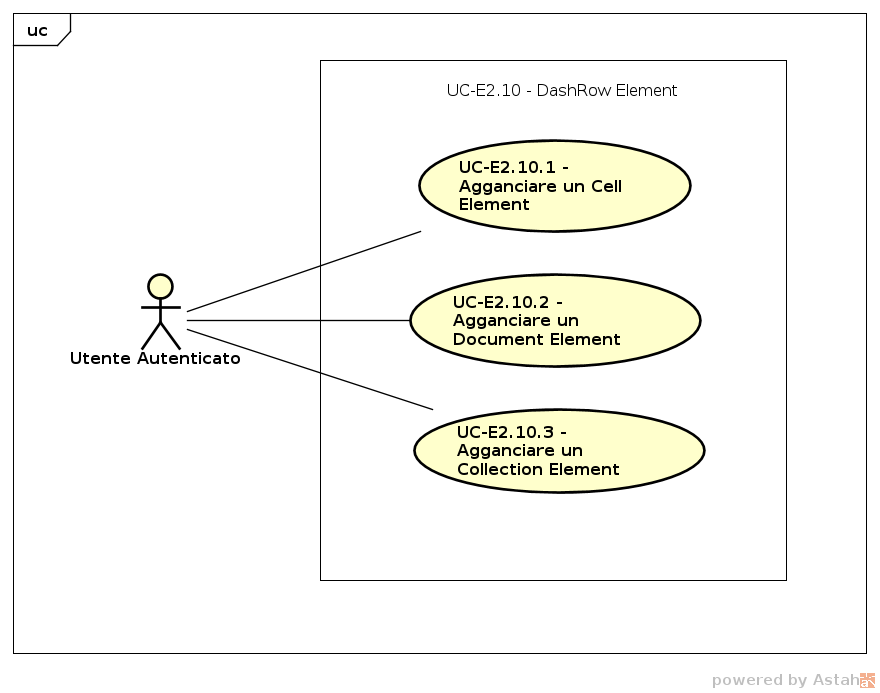
\includegraphics[width=12cm]{res/img/UCEditor/UC-E2.10-DashRowElement}
      \caption{UC-E2.10 - DashRow Element}
      \end{center} 
    \end{figure}

    %Tabella 
    \begin{center}
      \bgroup
      \def\arraystretch{1.8}     
      \begin{longtable}{  p{3.5cm} | p{8cm} } 
        
        \hline
        \multicolumn{2}{ | c | }{ \cellcolor[gray]{0.9} \textbf{UC-E2.10 - DashRow Element}} \\ 
        \hline
        
        \textbf{Attori Primari} & Utente Autenticato, Ospite, Membro, Admin, Proprietario \\ 
        \textbf{Scopo e Descrizione} & Definire la struttura di una ``row'' di una Dashboard in modo che l'utente possa scegliere quale configurazione applicare alla sua Dashboard \\ 
        
        \textbf{Precondizioni}  & Ci sia una Dashboard Element a cui far riferimento \\ 
        
        \textbf{Postcondizioni} & L'utente ha deciso la configurazione della riga della Dashboard \\ 
        \textbf{Scenario Principale} & 1. Agganciare un Cell Element (UC-E2.10.1)
2. Agganciare un Document Element (UC-E2.10.2)
3. Agganciare un Collection Element (UC-E2.10.3)
      \end{longtable}
      \egroup
    \end{center}
\subsubsection{UC-E2.10.1}

    %Tabella 
    \begin{center}
      \bgroup
      \def\arraystretch{1.8}     
      \begin{longtable}{  p{3.5cm} | p{8cm} } 
        
        \hline
        \multicolumn{2}{ | c | }{ \cellcolor[gray]{0.9} \textbf{UC-E2.10.1 - Agganciare un Cell Element}} \\ 
        \hline
        
        \textbf{Attori Primari} & Utente Autenticato, Ospite, Membro, Admin, Proprietario \\ 
        \textbf{Scopo e Descrizione} & Inserire nella riga della Dashboard una colonna rappresentante un Cell del DLS \\ 
        
        \textbf{Precondizioni}  & Ci sia una DashRow Element a cui riferirsi \\ 
        
        \textbf{Postcondizioni} & Nella Row del DSL viene aggiunta una colonna che visualizza un Cell
      \end{longtable}
      \egroup
    \end{center}
\subsubsection{UC-E2.10.2}

    %Tabella 
    \begin{center}
      \bgroup
      \def\arraystretch{1.8}     
      \begin{longtable}{  p{3.5cm} | p{8cm} } 
        
        \hline
        \multicolumn{2}{ | c | }{ \cellcolor[gray]{0.9} \textbf{UC-E2.10.2 - Agganciare un Document Element}} \\ 
        \hline
        
        \textbf{Attori Primari} & Utente Autenticato, Ospite, Membro, Admin, Proprietario \\ 
        \textbf{Scopo e Descrizione} & Inserire nella riga della Dashboard una colonna rappresentante un Document del DLS \\ 
        
        \textbf{Precondizioni}  & Ci sia una DashRow Element a cui riferirsi \\ 
        
        \textbf{Postcondizioni} & Nella Row del DSL viene aggiunta una colonna che visualizza un Document 
      \end{longtable}
      \egroup
    \end{center}
\subsubsection{UC-E2.10.3}

    %Tabella 
    \begin{center}
      \bgroup
      \def\arraystretch{1.8}     
      \begin{longtable}{  p{3.5cm} | p{8cm} } 
        
        \hline
        \multicolumn{2}{ | c | }{ \cellcolor[gray]{0.9} \textbf{UC-E2.10.3 - Agganciare un Collection Element}} \\ 
        \hline
        
        \textbf{Attori Primari} & Utente Autenticato, Ospite, Membro, Admin, Proprietario \\ 
        \textbf{Scopo e Descrizione} & Inserire nella riga della Dashboard una colonna rappresentante un Collection del DLS \\ 
        
        \textbf{Precondizioni}  & Ci sia una DashRow Element a cui riferirsi \\ 
        
        \textbf{Postcondizioni} & Nella Row del DSL viene aggiunta una colonna che visualizza un Collection
      \end{longtable}
      \egroup
    \end{center}
\subsubsection{UC-E2.11}
 

    \begin{figure}[H]
      \begin{center}
        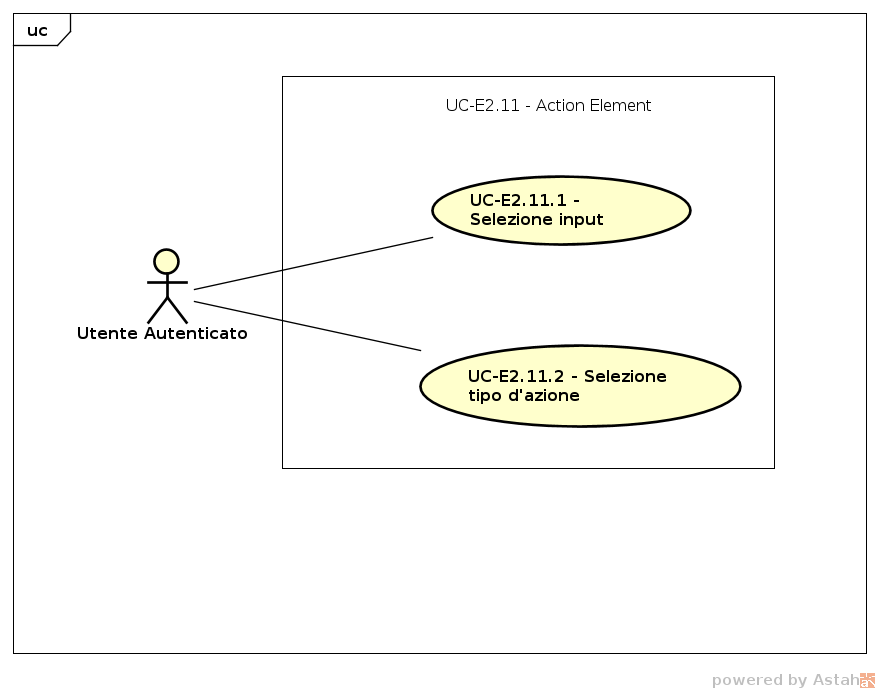
\includegraphics[width=12cm]{res/img/UCEditor/UC-E2.11-ActionElement}
      \caption{UC-E2.11 - Action Element}
      \end{center} 
    \end{figure}

    %Tabella 
    \begin{center}
      \bgroup
      \def\arraystretch{1.8}     
      \begin{longtable}{  p{3.5cm} | p{8cm} } 
        
        \hline
        \multicolumn{2}{ | c | }{ \cellcolor[gray]{0.9} \textbf{UC-E2.11 - Action Element}} \\ 
        \hline
        
        \textbf{Attori Primari} & Utente Autenticato, Ospite, Membro, Admin, Proprietario \\ 
        \textbf{Scopo e Descrizione} & Presentazione dell'Action del DSL nel quale si associa un'input ad una azione definita \\ 
        
        \textbf{Precondizioni}  & Ci dev'essere un documento o una collezione a cui si da riferimento \\ 
        
        \textbf{Postcondizioni} & Si \`e associato a quell'azione o a quel documento l'action desiderato \\ 
        \textbf{Scenario Principale} & 1. Selezione input (UC-E2.11.1)
2. Selezione tipo d'azione (UC-E2.11.2) 
      \end{longtable}
      \egroup
    \end{center}
\subsubsection{UC-E2.11.1}

    %Tabella 
    \begin{center}
      \bgroup
      \def\arraystretch{1.8}     
      \begin{longtable}{  p{3.5cm} | p{8cm} } 
        
        \hline
        \multicolumn{2}{ | c | }{ \cellcolor[gray]{0.9} \textbf{UC-E2.11.1 - Selezione input}} \\ 
        \hline
        
        \textbf{Attori Primari} & Utente Autenticato, Ospite, Membro, Admin, Proprietario \\ 
        \textbf{Scopo e Descrizione} & Selezionare il tipo di Action definite dall'Admin \\ 
        
        \textbf{Precondizioni}  & Ci dev'essere una Collection o un Document a cui fare riferimento \\ 
        
        \textbf{Postcondizioni} & L'Action viene legata all'elemento selezionata come input
      \end{longtable}
      \egroup
    \end{center}
\subsubsection{UC-E2.11.2}

    %Tabella 
    \begin{center}
      \bgroup
      \def\arraystretch{1.8}     
      \begin{longtable}{  p{3.5cm} | p{8cm} } 
        
        \hline
        \multicolumn{2}{ | c | }{ \cellcolor[gray]{0.9} \textbf{UC-E2.11.2 - Selezione tipo d'azione}} \\ 
        \hline
        
        \textbf{Attori Primari} & Utente Autenticato, Ospite, Membro, Admin, Proprietario \\ 
        \textbf{Scopo e Descrizione} & L'utente pu\`o definire l'azione legata all'Action \\ 
        
        \textbf{Precondizioni}  & C'\`e un'Action a cui fa riferimento \\ 
        
        \textbf{Postcondizioni} & L'utente ha definito quali azioni intraprendere eseguendo quell'Action 
      \end{longtable}
      \egroup
    \end{center}
\subsubsection{UC-E3}
 

    \begin{figure}[H]
      \begin{center}
        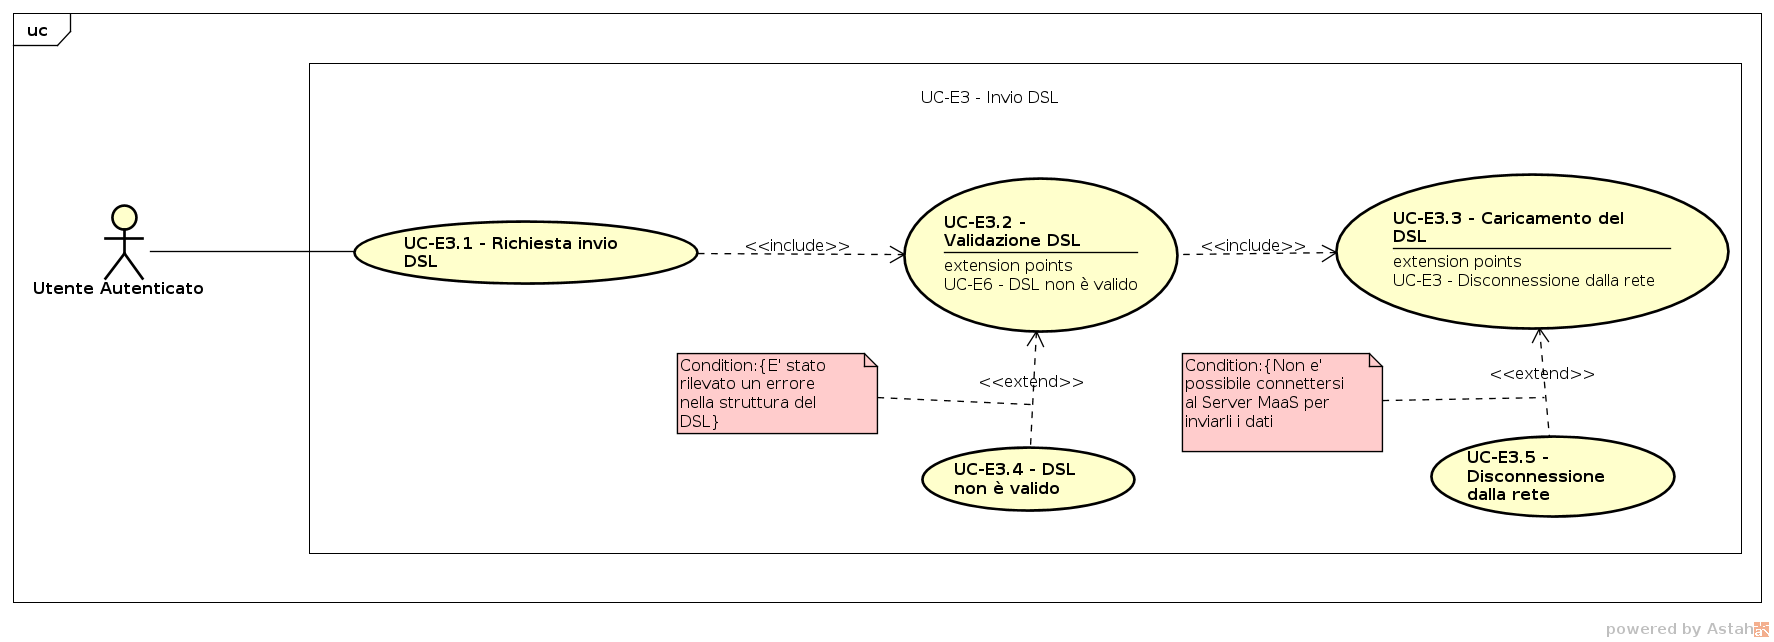
\includegraphics[width=12cm]{res/img/UCEditor/UC-E3}
      \caption{UC-E3 - Invio DSL}
      \end{center} 
    \end{figure}

    %Tabella 
    \begin{center}
      \bgroup
      \def\arraystretch{1.8}     
      \begin{longtable}{  p{3.5cm} | p{8cm} } 
        
        \hline
        \multicolumn{2}{ | c | }{ \cellcolor[gray]{0.9} \textbf{UC-E3 - Invio DSL}} \\ 
        \hline
        
        \textbf{Attori Primari} & Utente Autenticato, Ospite, Membro, Admin, Proprietario \\ 
        \textbf{Scopo e Descrizione} & Inviare la DSL al server per salvarla ed eseguirla \\ 
        
        \textbf{Precondizioni}  & L'utente visualizza l'editor \\ 
        
        \textbf{Postcondizioni} & Il DSL \`e stato caricato con successo sul MaaS ed eseguito \\ 
        \textbf{Scenario Principale} & 1. Richiesta invio DSL (UC-E3.1) 
      \end{longtable}
      \egroup
    \end{center}
\subsubsection{UC-E3.1}

    %Tabella 
    \begin{center}
      \bgroup
      \def\arraystretch{1.8}     
      \begin{longtable}{  p{3.5cm} | p{8cm} } 
        
        \hline
        \multicolumn{2}{ | c | }{ \cellcolor[gray]{0.9} \textbf{UC-E3.1 - Richiesta invio DSL}} \\ 
        \hline
        
        \textbf{Attori Primari} & Utente Autenticato, Ospite, Membro, Admin, Proprietario \\ 
        \textbf{Scopo e Descrizione} & L'utente chiede al programma dell'editor di eseguire tutte le operazioni necessarie affinch\`e ci sia l'invio del DSL al server e la sua esecuzione \\ 
        
        \textbf{Precondizioni}  & L'utente visualizza l'Editor \\ 
        
        \textbf{Postcondizioni} & Si sono avviate tutte le procedure dell'editor per eseguire i passi necessari per l'invio del DSL
      \end{longtable}
      \egroup
    \end{center}
\subsubsection{UC-E3.2}

    %Tabella 
    \begin{center}
      \bgroup
      \def\arraystretch{1.8}     
      \begin{longtable}{  p{3.5cm} | p{8cm} } 
        
        \hline
        \multicolumn{2}{ | c | }{ \cellcolor[gray]{0.9} \textbf{UC-E3.2 - Validazione DSL}} \\ 
        \hline
        
        \textbf{Attori Primari} &  \\ 
        \textbf{Scopo e Descrizione} & Al DSL creato vengano eseguiti tutti i controlli affinch\`e il parser possa interpretarli in maniera corretta \\ 
        
        \textbf{Precondizioni}  & L'utente ha fatto richiesta di invio del DSL \\ 
        
        \textbf{Postcondizioni} & Il DSL \`e stato correttamente validato e la sua correttezza \`e stata garantita \\ 
        \textbf{Estensioni} & 1. DSL non \`e valido (UC-E3.4)
      \end{longtable}
      \egroup
    \end{center}
\subsubsection{UC-E3.3}

    %Tabella 
    \begin{center}
      \bgroup
      \def\arraystretch{1.8}     
      \begin{longtable}{  p{3.5cm} | p{8cm} } 
        
        \hline
        \multicolumn{2}{ | c | }{ \cellcolor[gray]{0.9} \textbf{UC-E3.3 - Caricamento del DSL}} \\ 
        \hline
        
        \textbf{Attori Primari} &  \\ 
        \textbf{Scopo e Descrizione} & Inviare al server il DSL valido affinch\`e possa essere eseguito \\ 
        
        \textbf{Precondizioni}  & Il DSL deve essere valido \\ 
        
        \textbf{Postcondizioni} & Il DSL \`e stato correttamente caricato nel server MaaS \\ 
        \textbf{Estensioni} & 1. Disconnessione dalla rete (UC-E3.5) \\
      \end{longtable}
      \egroup
    \end{center}
\subsubsection{UC-E3.4}

    %Tabella 
    \begin{center}
      \bgroup
      \def\arraystretch{1.8}     
      \begin{longtable}{  p{3.5cm} | p{8cm} } 
        
        \hline
        \multicolumn{2}{ | c | }{ \cellcolor[gray]{0.9} \textbf{UC-E3.4 - DSL non `e valido}} \\ 
        \hline
        
        \textbf{Attori Primari} &  \\ 
        \textbf{Scopo e Descrizione} & Avvisare l'utente dove si trovano gli errori nel DSL definito \\ 
        
        \textbf{Precondizioni}  & Il DSL non \`e corretto \\ 
        
        \textbf{Postcondizioni} & L'utente \`e stato avvisato tramite un messaggio dove sono gli errori
      \end{longtable}
      \egroup
    \end{center}
\subsubsection{UC-E3.5}

    %Tabella 
    \begin{center}
      \bgroup
      \def\arraystretch{1.8}     
      \begin{longtable}{  p{3.5cm} | p{8cm} } 
        
        \hline
        \multicolumn{2}{ | c | }{ \cellcolor[gray]{0.9} \textbf{UC-E3.5 - Disconnessione dalla rete}} \\ 
        \hline
        
        \textbf{Attori Primari} &  \\ 
        \textbf{Scopo e Descrizione} & Avvisare l'utente dell'impossibilit\`a di effettuare il caricamento del DSL sul server \\ 
        
        \textbf{Precondizioni}  & Non \`e pi\`u possibile comunicare con il server MaaS \\ 
        
        \textbf{Postcondizioni} & L'utente \`e stato avvisato con un messaggio di errore dell'impossibilit\`a di caricare il DSL sul server MaaS 
      \end{longtable}
      \egroup
    \end{center}
